%!BIB program = bibtex
\documentclass[9pt, twocolumn, twoside, lineno]{pnas-new}
% Use the lineno option to display guide line numbers if required.

% PNAS研究论文模板
\templatetype{pnasresearcharticle} % Choose template 
% {pnasresearcharticle} = Template for a two-column research article
% {pnasmathematics} %= Template for a one-column mathematics article
% {pnasinvited} %= Template for a PNAS invited submission
% \usepackage{cite}
\usepackage{url}	
% 文章标题:“流域尺度的水资源利用体系:过渡框架和发展困局”
\title{Universal regime transition for water resources utilization in developing river basins}

% Use letters for affiliations, numbers to show equal authorship (if applicable) and to indicate the corresponding author
% 作者列表
\author[a, b]{Shuang Song}  % 宋爽,一作
\author[a, b, 1]{Shuai Wang}  % 王老师,通讯
\author[a, b]{Bojie Fu}  % 傅老师
\author[c, d]{Xutong Wu}  % 武旭同

% 机构列表
\affil[a]{ % 北师大地表国重
	State Key Laboratory of Earth Surface Processes and Resource Ecology, 
	Faculty of Geographical Science, 
	Beijing Normal University, 
	Beijing 100875, 
	P.R. China
}
\affil[b]{ % 北师大地理学部
	Institute of Land Surface System and Sustainability, 
	Faculty of Geographical Science, 
	Beijing Normal University, 
	Beijing 100875, 
	P.R. China
}
\affil[c]{ % 北大城环
	College of Urban and Environmental Sciences, 
	Peking University, 
	Beijing 100871, 
	P.R. China
}
\affil[d]{ % 中科院生态中心
	State Key Laboratory of Urban and Regional Ecology, 
	Research Center for Eco-Environmental Sciences, 
	Chinese Academy of Sciences, 
	Beijing 100085, 
	P.R. China 
}

% Please give the surname of the lead author for the running footer
% 领衔作者
\leadauthor{Song} 

% Please add a significance statement to explain the relevance of your work
% PNAS特有的“Significance陈述”,用不超过120个字来说明研究的意义和亮点
\significancestatement{
	% Authors must submit a 120-word maximum statement about the significance of their research paper written at a level understandable to an undergraduate educated scientist outside their field of speciality. The primary goal of the significance statement is to explain the relevance of the work in broad context to a broad readership. The significance statement appears in the paper itself and is required for all research papers.
	Water, a key resource to support the sustainable development of human societies, whose natural cycle has been modified by growing socio-economic processes. We propose a new method with an integrated index to detect water utilization regimes and applying it to the Yellow River Basin, a typical overexploited basin in China. After sketching changes of relationships between social development and water utilization within the Yellow River Basin, we summarized a universal transition framework. By predicting widespread development dilemmas, it can be a useful guideline for basins all around the world in their sustainable developing trajectories. 
}

% Please include corresponding author, author contribution and author declaration information
\authorcontributions{ % 作者的相应贡献
	Shuai Wang and Bojie Fu designed this research,
	Shuang Song performed the research and analysed data,
	Shuang Song, Xutong Wu wrote the paper.
}
\authordeclaration{ % 利益冲突陈述
	The authors declare no competing interests.
}

% 如果有共同一作的情况,则uncomment下面这行代码的注释
%\equalauthors{\textsuperscript{1}A.O.(Author One) contributed equally to this work with A.T. (Author Two) (remove if not applicable).}

% 通讯作者信息
\correspondingauthor{\textsuperscript{1}To whom correspondence should be addressed. E-mail: shuaiwang@bnu.edu.cn}

% 关键词,三到五个
% At least three keywords are required at submission. Please provide three to five keywords, separated by the pipe symbol.
\keywords{Regime shifts $|$ Human-water relationship $|$ Water resource management $|$ Water utilization $|$ Sustainable development} 

%tag 摘要
\begin{abstract}
	From agrarian to industrial societies, humans have harnessed ecosystems over rivers basins around the world, while using water resources as blood that sustains social developments. 
	Although relations between societies and water resources keep changing throughout, there is still lacking effective methods to detect related regimes of water resources utilization, with much fewer attempts to develop theoretical framework to explain their transitions as well. 
	Here, by integrating three important dimensions of water utilization (stress, priority and configuration), we develop an Integrated Water Resources Utilization (IWRU) Index at a basin scale to indicate regime shifts. 
	By applying this index to the Yellow River Basin, China, our results suggest three water utilization regimes in developing over half a century, whose shifts led by various but pervasive causes.
	Based on that, we summarized a universal transition framework which gives a sketch of relationships between human societies and their water utilization, as a useful guideline for big river basins to develop in a coordinated way.
\end{abstract}


\dates{This manuscript was compiled on \today}
\doi{\url{www.pnas.org/cgi/doi/10.1073/pnas.XXXXXXXXXX}}


\begin{document}

\maketitle
\thispagestyle{firststyle}
\ifthenelse{\boolean{shortarticle}}{\ifthenelse{\boolean{singlecolumn}}{\abscontentformatted}{\abscontent}}{}
% If your first paragraph (i.e. with the \dropcap) contains a list environment (quote, quotation, theorem, definition, enumerate, itemize...), the line after the list may have some extra indentation. If this is the case, add \parshape=0 to the end of the list environment.

% tag 引言第一段
% 水资源在人类世的重要性,是支持人类社会发展的基础。
\dropcap{W}ater, at “the centre of the planetary drama of the Anthropocene”, is not only essential for myriad Earth system processes, but also supporting development of human societies in various aspects. 
% TODO 这里增加三篇“大文章”参引
% 但同时, 人类的改造也深刻影响了自然水循环过程, 相关变化可能影响人水系统功能的不利转变,并带来发展困局。
However, human's modification has profoundly influenced the water cycle which may lead adverse changes to functions of human-water systems, resulting in various development dilemmas \cite{gleesonIlluminatingWaterCycle2020,cummingLinkingEconomicGrowth2018}.
% TODO 这里增加参考文献,人类对水循环的改造 
% 大河流域常是经济和文明发展的中心,同时也是面临人类世压力挑战的主要地区,亟需综合水资源治理以实现可持续发展。
Facing major challenges in the Anthropocene, many of the world's big river basins, also hot spots of economy and civilization, are urgently in need for integrated water resources management toward sustainability \cite{bestAnthropogenicStressesWorld2019}. 
% 因此理解人类社会发展与水资源利用的复杂关系,对此有帮助。
Therefore, understanding the complex relationship between human societies, water resources utilization and their transitions provides underlying supports for developing in a coordinated and sustainable way at a basin scales.

% tag 引言第二段
% Regime 和 Regime shift 的定义。
Regime is a stable state of system’s structure and function, whose large and persistent changes may lead to substantive impacts on the outcomes of system with widespread cascading effects, defined as regime shifts \cite{rochaCascadingRegimeShifts2018, schefferCatastrophicRegimeShifts2003, schefferCatastrophicShiftsEcosystems2001}.
% 人水系统中的水资源功能
Water have several key functions within a human-water system, the most important of which is supplying for human societies in further developments based on water utilization. 
% 水资源利用 regime shift
However, interplayed human interference, involving water withdrawal, dam constructions and water managements have significantly changed water functions and induced changes in water use
\cite{falkenmarkUnderstandingWaterResilience2019}.
% 稳态转换随着社会发展增加
These gradual or abrupt drivers triggered regime shifts as societies' development strengthen their interlinks to water utilization and deepening dependences on them.
% TODO 这里需要安排参考文献,稳态转换的触发方式,随着社会发展更多
% Regime 过渡性的存在
As a result, most large river basins had gone through water utilization regimes of accelerated exploitation, over-exploitation, and integrated management, for which it is a reasonable assumption that there is a general transition pattern. 
% TODO 这里需要安排参考文献,大河流域的发展历程
% 过渡性有助于理解流域存在的问题
Sketching the transition of water utilization regimes, therefore, can help to understand and predict developing trajectories of basins, which are crucial for integrated management and coordinated development towards sustainability.
% 对过渡性的研究还很少
Despite pervasiveness, there is still lacking of effective method to distinguish the water utilization regimes and detect regime shifts, with much fewer attempts to develop theoretical models to explain their transitions as well. 

% Tag 引言第三段
% 前人已经从不同维度刻画了人水关系.
Development of societies by using water resources has been going on for at least thousands of years. Although its regime shifts and transition phases are not fully understood yet, features of water utilization has been depicted and studied from different perspectives.
% 首先,因为水资源的稀缺性和全球用水量的增加,受到最广泛关注的是人类社会面临的水资源压力。
Firstly, water stresses are of increasing importance and concerns because of scarcity.
Greater water utilization stresses had become a major constraint to development, because of significant increment in water withdrawals and larger shares of inflexible water use during the last century, while store of water resource in reservoirs are helpful to relief of
\cite{postelHumanAppropriationRenewable1996, greveGlobalAssessmentWater2018, qinFlexibilityIntensityGlobal2019}.
% 其次,随着工业迅猛发展和生态建设的需要,社会对水资源的利用的倾向性也发生了转变。
Secondly, as the need of industry, services and ecology developments, priority of water utilization changed with. 
Despite a major water utilization of agricultural irrigation dominating most river basins, there are noticeable growths in economy profits of industry or services and their priority in water consumption, leading potential conflicts between different sectors
\cite{liuWaterScarcityAssessments2017, florkeWaterCompetitionCities2018}.
% 最后,由于水的可用性本质上是区域问题,水资源利用的格局也很重要
Thirdly, since water distribution and utilization are inherently regional concerns where all regions attempt to develop themselves by economically competitive sectors, configuration also plays as an important aspect.
% 全球总的取水量很少,但缺水地区很多
While only 10\% of available water is withdrawn on global average, about 30\% of population settles in highly water-stressed regions with vary dominated water demands
\cite{wadaWedgeApproachWater2014, okiGlobalHydrologicalCycles2006}.
% 此外,人类活动还在改变这一格局
Human activities further affect this configuration, as positive impacts mostly occur in upper regions whereas aggravated downstream, though most governments are trying to control this situation. 
\cite{veldkampWaterScarcityHotspots2017}. 
% 总的来说,上述三个维度试图解答与水资源利用有关的三个重要问题 “还有多少水资源可以利用”,“把水资源用在什么”
Taken together, existing researches have evaluated the three dimensions of water resource utilization regarding a series of crucial questions: ``How much water resources?'', ``How to use them?'' and ``Used for whom or in where?''.
% 将三种视角结合,就是“水资源利用体系”。
As these dimensions haven't been well integrated by quantitative methods, however, there is still lacking a coherent interpret of regime shifts regard to social development and water utilization.


% tag 引言最后一段
% 这里我们整合了三个方向,提出了描绘流域人水关系的指数
Here, by integrating three above mentioned dimensions of water utilization, we develop an Integrated Water Resources Utilization (IWRU) Index at a basin scale to give a sketch of relationships between human societies and their water utilization (Figure~\ref{fig:framework}).
% 使用案例研究
Then, by applying this index to the Yellow River Basin, China, we analysed water utilization regimes and their shifts in this typical basin of anthropogenic impacts, with change points detection and contribution decomposition methods following.
% 指出发展困局
In addition, combining data analysis, we identify drivers of the regime shifts. 
% 最后总结出一般性框架
Finally, refer to the existing theories, we summarized a universal transition framework of water utilization regimes, which can be a useful guideline for basins to predict development dilemmas and to develop in a coordinated way.


\begin{figure*}%[htbp]
	\centering
	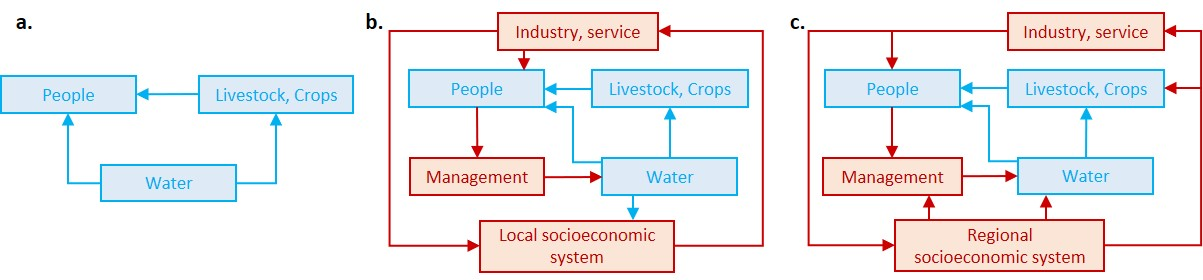
\includegraphics[width=0.8\linewidth]{../../figures/main/framework.jpg}
	\caption{
		A framework for understanding the changing relationship between watershed development and water resources.
		% 图A是水资源利用的三个维度。每个维度都有两个极点(红色字表示),指示水资源利用在该轴上的两个变化方向。
		\textbf{A,} three dimensions (stress, priority and configuration) of water resources utilization. Each dimension has two poles (denoted in red) which indicates the two potential directions of water resources utilization changes along that axis. (1) Stress of water utilization shifts between scarcity of water resources and abundance of water resources, which means there is shortage of water supply or not. (2) Priority of water utilization can move between a provisioning part or a non-provisioning one, indicating how much water were used in food supporting to human societies. (3) configuration can move between balanced or lopsided, when allocation of water resources between different sectors or regions changed. We presume that water utilization regimes equally weighted by these basic dimensions, whose combination can highly relate to basin development. 
		% 图B是将三个维度结合后的变化情况。因上述三个维度随着社会发展而不断变化,其组合的水资源利用状态也不同。这个过程中当突变发生时,可能标志着水资源利用发生了稳态转换,因此我们需要一个指标来监测其变化。
		\textbf{B,} the changes after combining the three dimensions. Because the above three dimensions are changing with the development of society, their combined water resource utilization status is also different. When abrupt transitions occur during this process, they may indicate a regime shift in water utilization, so we need an indicator to monitor this change.
	}
	\label{fig:framework}
\end{figure*}


\section*{Results}
\subsection*{Water utilization regimes}

\begin{figure}[h!]
	\centering
	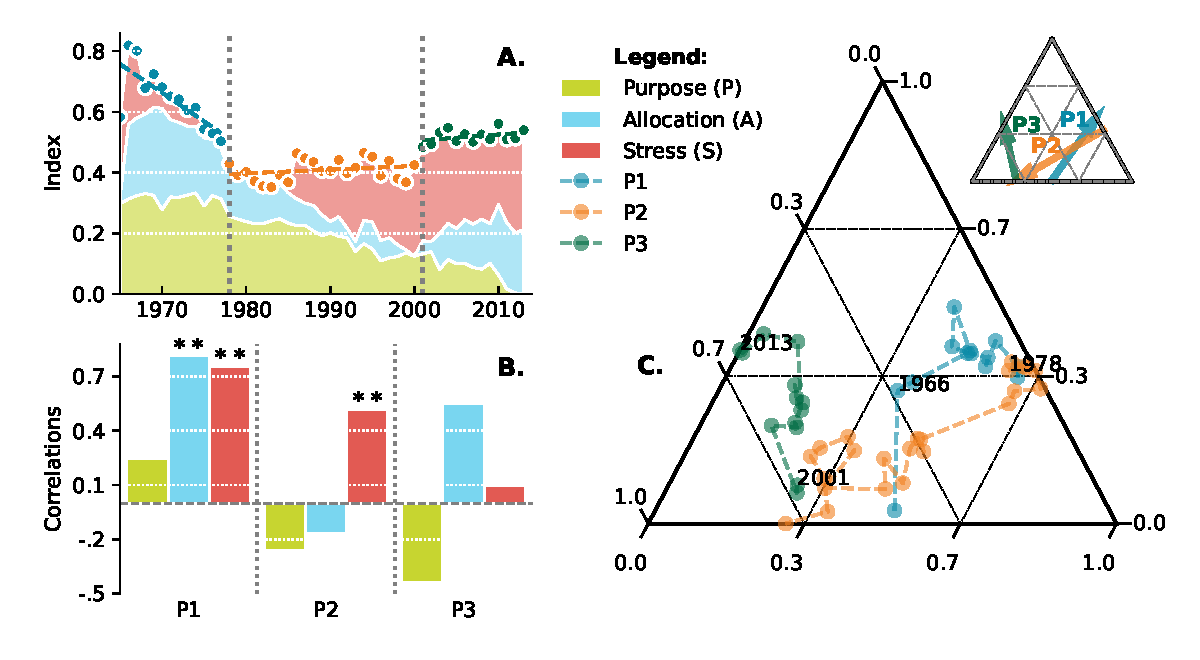
\includegraphics[width=\linewidth]{../../figures/main/index.pdf}
	\caption{Changes of the IWRU index. 
	\textbf{A,} two change points in 1978 and 1994, three periods were detected in changing trend of the IWRU.
	\textbf{B,} changes of IWRU in three periods have various slopes, while the second period have a negative growths rate.
	\textbf{C,} changes of the IWRU within three periods, which have different main contributors.
	}
	\label{fig:IWRU}
\end{figure}

% 这一节主要展示IWRU的变化趋势和WUR的划分
With two significant points, the trend of IWRU index are detected into three periods, whose slopes of changing are various and mainly contributed by different dimensions (stress, priority or configuration of water utilization, see \textit{Methods}) (Figure~\ref{fig:IWRU}).
% 接下来分句介绍每个阶段的特征
% 第一阶段
In the first period (P1, 1965-1978), the IWRU index had a rapidly increasing and the lightening of water stresses made the most striking contribution (+0.722 change contribution and 83.7\% net contribution), while priority and configuration of the water utilization had slight negative contribution (-0.048 and -0.09 in change contributions, 5.6\% and 10.7\% in net contributions, respectively).
% 第二阶段
In the second period (P2, 1979-1994), the IWRU index experienced a slight drop, despite positive contributions of priority and configuration of water utilization (+0.352 and +0.279 in change contributions, 22.0\% and 27.8\% in net contributions respectively), because of increasing stresses on water resource playing a larger negative role (-0.636 change contribution and 50.2\% net contribution). 
% 第三阶段
However, as the further increasing of positive contributions of water utilization priority (+0.485 change contribution and 36.1\% net contribution) and configuration (+0.515 and 38.3\%, corresponding), and decelerations of water stresses (-0.344 change contribution, 46\% less than P2) in the third period (P3, 1995-2013), a positive growth of the IWRU returned.
% 总而言之,每个阶段都由水资源利用的不同维度提供最大的正向作用
As a result, each period has a different most striking positive contributor to IWRU: P1 is stress; P2 is priority; and P3 is configuration.

% 用水三个维度的组合呈现出阶段特征明显
Combining these three dimensions' net contribution (differ from change contributions, see \textit{Methods}) to IWRU further, ratios of the contributions of the three dimensions clustered clearly by different time periods, indicating three regimes (Figure~\ref{fig:phases}).
\begin{figure}%[htbp]
	\centering
	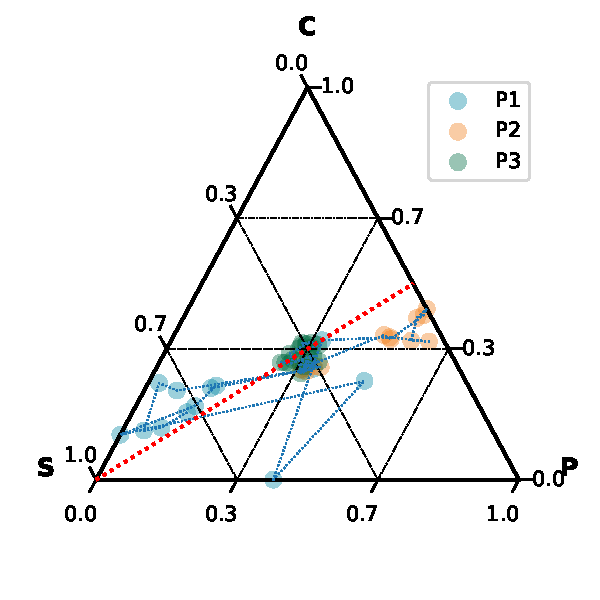
\includegraphics[width=0.9\linewidth]{../../figures/main/phases.pdf}
	\caption{Combination of net contributions regards three dimensions in different periods (S: stresses; P: priority; C: configuration). The closer a point to an angle of the triangle, greater the proportion of the net contribution of this dimension.
	The red indicator line in this ternary plot denotes 1:1 contributions between priority (P) and configuration (C). When the points are bellow this line, the net contribution ratio of configuration is lower than that of priority, and vice versa.}
	% 由于阶段一的点位于该线上方,L的净贡献比例多于P,而第二阶段的点则恰好相反。
	\label{fig:phases}
\end{figure}
% 第一阶段到第二阶段
At the very beginning (1965) and throughout the whole P1, water utilization regime dominated by high stresses. After then, it experienced a shift to low stresses since 1978, with a change in the proportion of net contributions between priority and configuration, too.
% 第三阶段集中
Finally, the net contribution of three dimensions were much similar in P3 (32.91\%, 31.87\% and 35.21\% for priority, configuration and stress respectively), making the points highly concentrated at the centre of the ternary diagram in that period.


%tag 结果2
\subsection*{Differences between water utilization regimes}
% 在不同的维度下各阶段进行对比,可以发现不同的水资源利用体系间存在明显差异。
The differences between the water utilization regimes are reflected in changes of all three dimensions.
\begin{figure*}%[htbp]
	\centering
	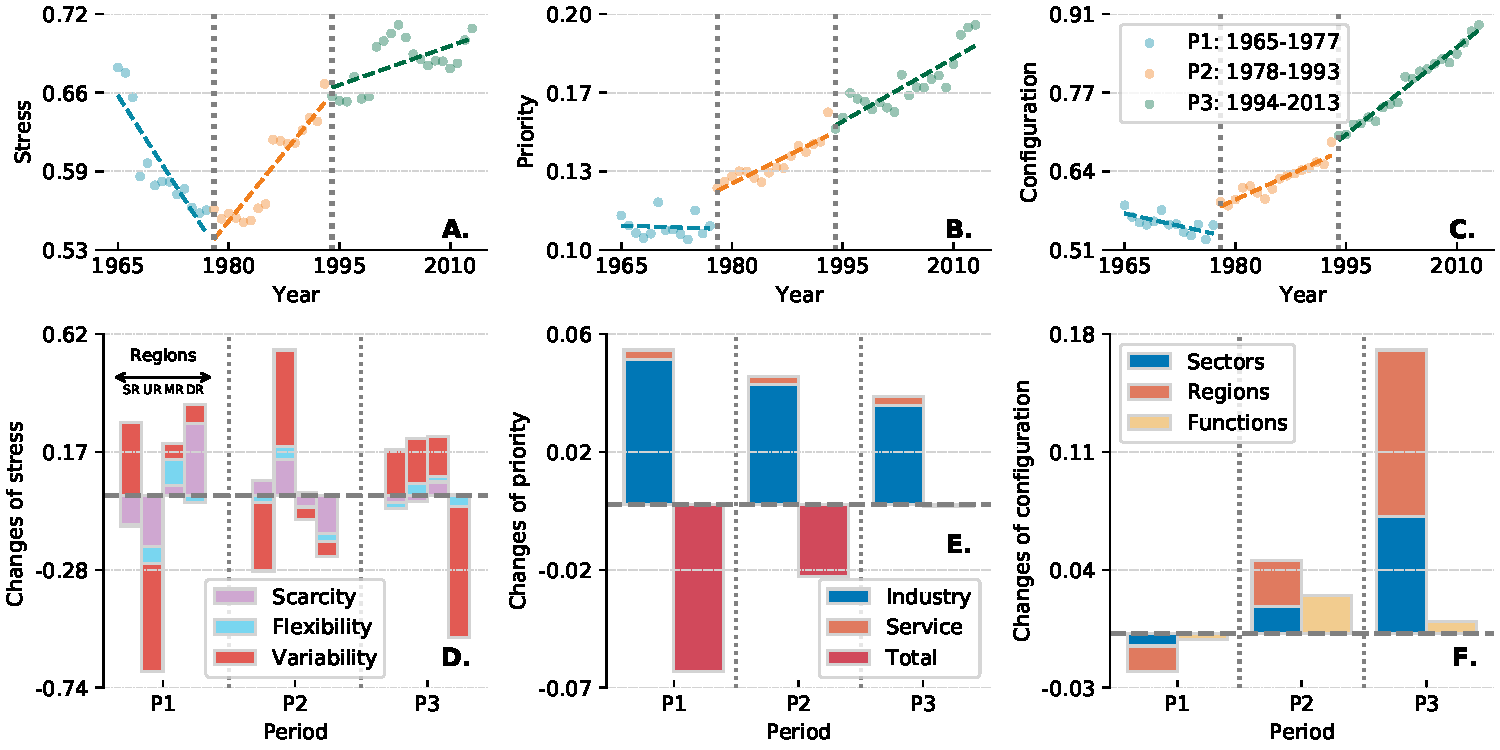
\includegraphics[width=\linewidth]{../../figures/main/dimensions.pdf}
	\caption{
		Changes in different dimensions of water resources utilization regimes and their main contributors.
		\textbf{A,} changes of water utilization stress, indicated by unstandardized scarcity-flexibility-variability water stresses index (SFV-index, see \textit{Methods} and \textit{SI Appendix} Method S4).
		\textbf{B,} changes of water utilization priority, indicated by non-provisioning water shares (see \textit{SI Appendix} Methods S4).
		\textbf{C,} changes of water utilization configuration, indicated by unstandardized distribution information entropy index (\textit{Methods} and \textit{SI Appendix} Method S4).
		\textbf{D,} Main impact factors to water utilization stresses in each period or region, and their change contributions to unstandardized SFV-index.
		\textbf{E,} Main impact water uses to water utilization priority, and their change contributions to non-provisioning water shares.
		\textbf{F,} Main impact factors to water utilization configurations, and their change contributions of related unstandardized distribution information entropy index (\textit{Methods} and \textit{SI Appendix} Method S4).
		}
	\label{fig:dimensions}
\end{figure*}
% 从阶段一到阶段二,水资源压力的变化最为明显
Moving from the regime in P1 to P2, the most striking change is the reversal of the trend in water utilization stress(Figure~\ref{fig:dimensions}A), which is determined by a combination of scarcity, flexibility and variability (Figure~\ref{fig:dimensions}D and \textit{SI Appendix} Method S4).   
% 1. 水资源丰富,耗水量少且灵活用水
In the P1, natural surface water resources were rather abundant with fewer water consumptions (\textit{SI Appendix} Fig. S3) and most of which were flexible water utilization (\textit{SI Appendix} Fig. S4). During the P1 and even P2, however, water consumption increases rapidly and natural surface water resources decreases at the same time, making water increasingly scarce. Opposite effect to that, numerous reservoirs built reduced the variability of water resources by boosting storage capacities, but there are much fewer reservoirs built in P2 (\textit{SI Appendix} Fig. S5). As a result, water utilization stress decreases during P1, but begins to rise rapidly in P2.

% 另一方面,P2-P3,持续变化的水资源利用倾向与格局
On the other hand, as the most positive contributors to the IWRU index in P2 and P3 separately, priority (Figure~\ref{fig:dimensions}B) and configuration (Figure~\ref{fig:dimensions}C) of water utilization were keeping to enlarge their impacts. 
% 首先是用水比例的变化
Representing priority of water utilization, increasing non-provisioning share of water utilization were mainly contributed by larger industrial water consumptions and minor total water uses, while their influences are weakening (Figure~\ref{fig:dimensions}E).
% 再讨论用水格局的变化
However, configuration of water utilization, whose contributions to the IWRU are increasing, were mainly benefited from decreasing differences in the amount of water resources used, both intersectoral and regional (Figure~\ref{fig:dimensions}F).


% tag 结果3
\subsection*{Drivers of water utilization regime shifts}

\begin{figure}%[htbp]
	\centering
	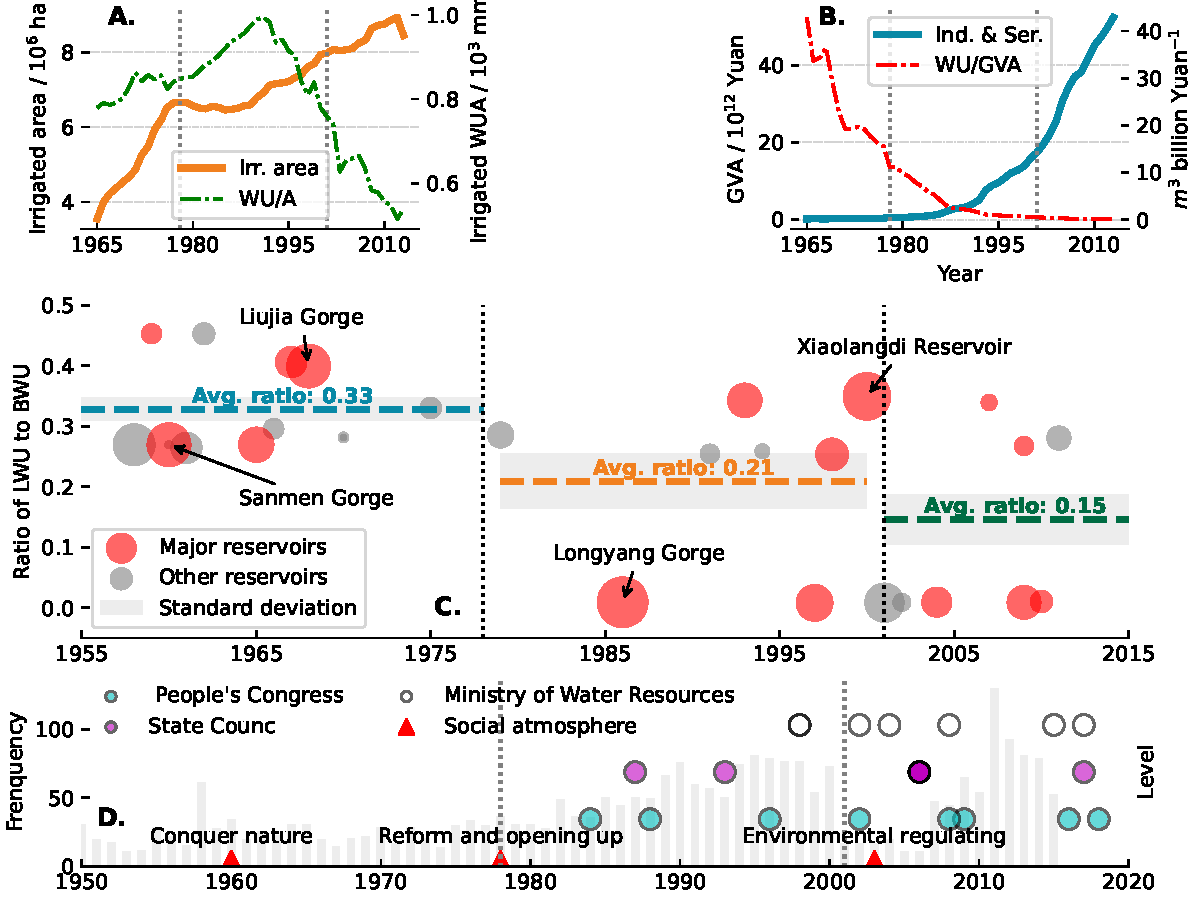
\includegraphics[width=\linewidth]{../../figures/main/causes.pdf}
	\caption{
		Drivers of water utilization regime shifts: economy growths, efficiency changes, and management practices.
		\textbf{A.} Changes of total irrigated area, and water consumptions in per unit of area (\textit{SI Method} S2).
		\textbf{B.} Changes of gross values added (GVA) of industry and services, and their water use density (WUI) respectively (\textit{SI Appendix} Method S2).
		\textbf{C.} Constructions' finished time of each new reservoir and their located regions' water use percentages in basin's total water use (WU), at that time. Red ones denote hub reservoirs in the basin, which plays a role in bainsal integrated water management. Size of the points indicates their magnitude of water storage capacities. Some important or special reservoirs' name denoted: (1) Xiaolangdi reservoir and Sanmen Reservoir were constructed mainly responsible for managing sediments of the Yellow River. (2) Liujia Gorge, Longyang Gorge, were constructed mainly responsible for managing water flood discharge and storage. These marked reservoirs, therefore are significant for the entire basin, far crucial than regional development.
	}
	\label{fig:Causes}
\end{figure}

Some main drivers caused the above changes of water utilization regime.
% 经济总量提升导致资源耗竭的加速。
(1) The expansion of irrigated area and the economic growth of industry and services are keys to the changes in the priority of water utilization between P1 and P2 (Figure\ref{fig:Causes}A). During the P1, irrigated agricultural area in the Yellow River basin expanded rapidly at a rate of $0.25*10^6 ha/yr$, and irrigation water was the dominant utilization way ($81.56\%$ of the total water use in 1965, and $83.17\%$ in 1978, see \textit{SI Appendix} Fig. S6). Entering P2, however, while the expansion of irrigated area stalled, industry and services gradually took off and took up more water resources (Figure\ref{fig:Causes} B), leading to $8\%$ reduction of proportion of irrigation water (\textit{SI Appendix}).

% 用水关系的变化
(2) During the P3, irrigation had noticeable changes in its efficiency, whose water consumptions were reduced but still dominant. Although irrigated area resumed expansion, and both industry, urban services were boosting their gross added values (GVA), water use density (WUI) experienced significant declines and reached the lowest points (Figure\ref{fig:Causes}A and Figure~\ref{fig:Causes}B). It means, water utilization ways  have changed, along with technological solutions and a range of water conservation practices. As a result, the differences between the sectors of water use reduced while the total water consumption remains stable, during the P3 (\textit{SI Appendix} Fig. S6).

% 不断变化的管理模式。
(3) Changing water management practice contributed throughout all three periods. In the P1, most of the reservoirs are built in regions with high water demands, as ratio of regional water use and basinal water use for each new reservoir are significantly higher (Figure~\ref{fig:Causes}C, p<0.01). In the P2, on the other hand, the number of new reservoirs decreases significantly with little increment of total storage capacities (\textit{SI Appendix} Fig. S5). Entering the P3, however, the number of new reservoirs are even much higher than that in the P1, and most of them were built in regions with lower ratio of regional water use and basinal water use (Figure~\ref{fig:Causes}C and \textit{SI Appendix} Fig. S5).

% tag 讨论
\section*{Discussion}

\subsection*{Interpret of regime shifts within YRB}
% 我们发明的指数能将三个维度的变化捕捉到。
The IWRU index captures, with three dimensions (stress, priority and configuration), the complex human-water feedbacks that links social development and water resources utilization. 
% 我们为的研究结果表明,黄河流域能被识别为三个明显的稳态
Our results show that three distinct regimes of water utilization within YRB, which have been driven by different causes regarding the three above dimensions.
% 在第一个稳态时期(即P1: before 1978),黄河流域农业的GDP贡献曾达到,超过经济效率通常更高的工业和服务业。
Before 1978, the contribution of agriculture in the YRB to GDP was nearly a half (46\% in 1965), much higher than that of industry or services (33\% and 26\% in 1965, respectively see \textit{SI Appendix} fig. S8). 
% 考虑到彼时下游的工业用水尚未从黄河取水,且按省估计的夸张,这个数字仍远远低估了黄河流域的社会发展对农业的依赖。
Given that downstream industrial water had not depended on Yellow River yet, and the provincial estimates are exaggerated in industrial or services GDP (\textit{SI Appendix} Methods S3), this figure still greatly understates the dependence on agriculture for social development then.
% 因此那时候,黄河流域主要管理组织黄河水利委员会()的主要工作之一是成立水利机构从事水利建设,而新建设的水库也多分布于高需水的区域。
At that time, one of the main tasks of the Yellow River Conservancy Commission (YRCC), therefore, was to set up agencies for water infrastructure (\textit{SI Appendix} Table S2), and the new reservoirs were mostly distributed in regions with high water demands (Figure~\ref{fig:Causes} C). 
% 结果是,该稳态的主要特征表现为灌溉用水的迅速扩张,以支持农业发展。
As a result, this regime is characterized by a rapid expansion of irrigation water to support development of agriculture.

% 但因水资源危机的到来,上一制度与扩张性的农业发展随之结束,此时黄河耗水量已占天然径流量的约77%。
% 1972年,黄河首次断流19天,断流长度达310km,并连续多年断流。
The regime, however, nearly came to an end with the water resource crisis, as the water consumption of the Yellow River had accounted for about 80\% of the natural runoff. In 1972, the Yellow River was cut off for the first time with a length of 310 km for 19 days, and continued to be cut off for many years since then (\textit{SI Appendix} Fig. S9). 
% 来到1978年的制度时,黄委会领导改组,并接到水利部的批示,要求恢复和加强水文和流域管理相关的工作,
Came to the regime since 1978, the YRCC undergone a reorganization and received instructions from the Ministry of Water Resources (called Ministry of Water Resources and Electric Power then) to resume and strengthen work related to hydrology and basin management in YRB.
% 自此,稳态农业的扩张趋势得到了遏制(图causes),大部分流域尺度及以上的法律规章从此开始逐步推行,并在1987年提出了影响深远的“87分水方案”,为流域内各省份限定了可引水量
Since then, the expansion trend of agriculture has been constrained in this regime (Figure~\ref{fig:Causes}A), while the importance of industry began to increase with the opening up of Chinese market. In addition, most laws and regulations have been successively implemented (\textit{SI Appendix} Table 3). For an example, the far-reaching “87 Water Diversion Scheme”, which was put forward in 1987, limited the amount of water withdraw for each province as a constant in the YRB.

% 下一次稳态转换直到1993年左右才由用水效率的显著提升而带来。
The next regime shift was not occurred by a significant increase in water use efficiency in about 1993. 
% 此时在经历了十余年发展后,经济的重心已经倾向了工业和服务业,农业在GDP中的比重此时只占23%。
After more than a decade of development, the focus of economy had shifted to industry and services whose contribution of GDP in YRB are 45\% and 31\%, while agriculture accounting for only 23\% (\textit{SI Appendix} Fig.S8).
% 经济增长的同时,工业用水需求也迅速增加,两者推动了用水效率低下的农业实施节水改革。
A rapid increase in industrial demand for water has been accompanied by economic growth, which had led to water-saving reforms in inefficient agriculture. As a result, water use efficiency improved significantly in both agriculture and industry during the third regime (Figure~\ref{fig:Causes}A and Figure~\ref{fig:Causes}B), with engineered water-efficient irrigation reaching nearly half (48.6\%) of the total irrigated area (\textit{SI Appendix} Fig. S7), allowing the average water consumption per unit of irrigated area to drop about tenfold (Figure~\ref{fig:Causes}A).

In short, agricultural expansion, industrial services expansion, water resources management, as well as scientific and technological progress and water use efficiency improvement, have driven the YRB to change regimes twice between 1965 and 2013, which had been along with social development in different aspects and can be interpreted by a transition process.

\subsection*{Transition framework of water utilization}

\begin{figure*}[thbp]
	\centering
	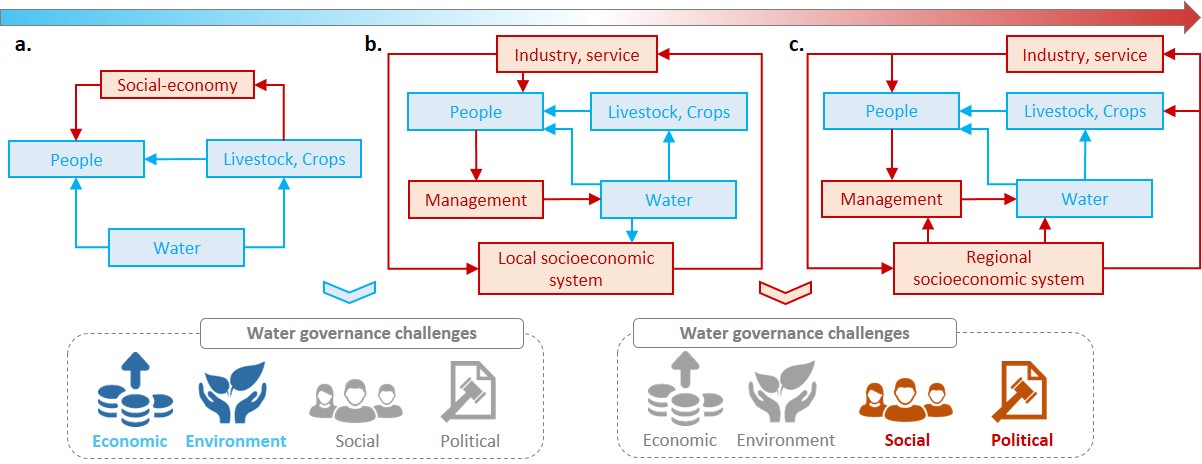
\includegraphics[width=\linewidth]{../../figures/main/transition.jpg}
	\caption{
		Transition framework of the water utilization regime towards nature-society dualistic water cycle.
		\textbf{A. Natural cycle:} As an indispensable provisioning resource, the main functions of water resource is to support crop, livestocks and human-beings, which are the basic ecological services.
		\textbf{B. Local cycle:} With local socio-economic systems developing, industry and services (also known as the secondary and the tertiary industry) calling for further water consumptions.
		However, as their ecological services generated through the socio-economic cycle, water resource plays a non-provisioning role. What's more, better organized socio-economic system and developed technology gives humans abilities in better managing water resources, with intensive intervention in the natural water cycle. 
		\textbf{C. Regional cycle:} Entering this phase, with further developed and economically efficient industries and services, trade-off between whose water demands with provisional water demands becomes prominent. Rather than determined by local socio-economic systems, water withdrawals and management act as considerations within the entire basin more, therefore. 
	}
	\label{fig:summary}
\end{figure*}

% 上述过渡过程与稳态转换的关联可能是普遍的
The association between the above transition process and the regime shifts may be pervasive.
% 普遍存在的稳态转换可以由渐变或突变造成,而人类压力在世界范围内都是稳态转换最重要的驱动因素之一。
Widespread regime shifts in a human-water system can be triggered by accumulation of gradual changes, where increasing anthropogenic pressure are among the most important drivers \cite{rochaCascadingRegimeShifts2018,falkenmarkUnderstandingWaterResilience2019}. 
% 而随着人类干预的加深,水循环出现了自然-社会二元结构,主导当前人水系统的互馈过程。
At the same time, human society has become more and more dependent on water utilization as it further develops, modifying natural water cycles by socio-economic processes \cite{gleesonIlluminatingWaterCycle2020,dibaldassarreSociohydrologyScientificChallenges2019}.
% 与社会-自然二元水循环理论
This social water cycle has linked to the natural water cycle through water utilization, forming a closed chain of interdependence, interconnection and mutual influence, which is consistent with nature-society dualistic water cycle theory
\cite{qinTheoreticalFrameworkDualistic2014,liuDualisticWaterCycle2010}.
% 我们的研究结果表明,与社会-生态系统的过渡过程类似,水资源利用体系的变化也存在类似稳态转换的阶段性特征,并最终呈现出自然-社会二元结构。
According to our results, regime shifts of water utilization, with changing in three related dimensions induced by social development, are of the most important characteristics towards natural-social dualistic cycle
\cite{cummingImplicationsAgriculturalTransitions2014,cummingLinkingEconomicGrowth2018}.
% 因此,我们在总结黄河流域变化过程的基础上,进一步概念化了水资源利用制度的过渡框架。
As such, we summarized a universal transition framework of the water utilization regimes here, which conceptualizes a general trajectory towards a natural-social dualistic water cycle (Figure~\ref{fig:summary}).


% 水资源利用制度包括压力、倾向性、格局三个重要因素,三个指标在过渡框架中随着不断变化。
Throughout the transition towards dualistic water cycle, three dimensions of water utilization regime are various in discipline of changes. 
% 水资源压力
(1) Firstly, although stresses on water resources increases when economic expansion boosting water demands, socio-economic progress can response to resource scarcity by better management or efficiency. Water resources were becoming more scarce in the YRB from P1 to P3 (\textit{SI Appendix} Fig. S3). However, water utilization stresses changes a lot rather than always increasing with, because of expansions of farmland, constructions of reservoir, and the increased water use efficiency were all responses and played roles in different aspects (Figure~\ref{fig:Causes}). Since the scarcity of water resources is directly perceptible and sensitive for utilization, its stresses on societies is one of the most striking drivers to regime shifts within human-water systems \cite{qinFlexibilityIntensityGlobal2019}.
% 水资源倾向性
(2) Secondly, the non-provisioning part of water demands growths with secondary and tertiary industries developing, leading priority of water utilization continually tilted to the socio-economic part. As original region of Ancient Chinese Civilization, the Yellow River Basin used to be dominated by agricultural but in its way to an energy industry zone now \cite{WillEnergyBases}. As a result, saving water consumption in agriculture and making concessions for industry and energy is widely recognized as solutions for the competing \cite{xiangWillEnergyIndustry2016,bebbWaterRightsTransfers2011}. Anyhow, this changes of priority reflect a truth that growing socio-economic parts are responding to scarcity of water resources and contributing to regime shifts.
% 水资源格局
(3) Last, with tighter socio-economic links and comparative advantages between regions and sectors, the geographic scope of water resource supply and demand allocation is expanding, leading to changing configurations of water utilization. In the Yellow River Basin, the gap in water consumptions between regions and sectors are narrowing, as the result of a carefully designed allocation \cite{wangThirtyYearsYellow2018}. However, the configuration of water utilization is determined on the basis of regional and sectoral economic contexts and development trajectories\cite{wangThirtyYearsYellow2018}. The changes in water utilization configurations along with regime shifts, therefore, are the outcomes of feedback loops within complex human-water systems.

% 综上所述
By combining the above three dimensions, these changes gradually transformed water utilization regimes in a ``natural cycle'' (Figure~\ref{fig:summary}A) to one in local or regional cycle (Figure~\ref{fig:summary} B and C), towards a natural-society dualistic water cycle. In addition to the Yellow River Basin, which is the focus of this study, human-water relations in major river basins around the world can be explained by the framework. For examples, Indus River, Mississippi River, and Danube River, whose water utilizations have all gone through a relatively natural regime, rapid developments and integrated management regimes. \cite{bestAnthropogenicStressesWorld2019,cummingResilienceBigRiver2011}. In summary, our proposed transitional framework for the nature-society dualistic water cycle is universal in interpreting regime shifts of water utilization.

\section*{Dilemmas and future directions}
% 对于可持续科学,认识这种稳态的变化很重要
For sustainability scientists, recognizing that different regimes of water utilization regarding different water utilization regimes has important implications for social development and river basin management.
% 不同的流域位于过渡的不同阶段,面临的问题也存在区别,主要包括资源陷阱和结构陷阱两类。
At different transition phases, however, basins may face to various development dilemmas in water utilization, leading an unsustainable trajectory. 
% 资源陷阱和失配,导致崩溃
Like social-ecological systems and other complex systems, coupled human-water system may collapse under the stresses reached the tipping point or structural mismatches 
\cite{reyersSocialEcologicalSystemsInsights2018,cummingQuantifyingSocialEcologicalScale2020,wangCOSUSTMs0530Review}. 
% 转型应对陷阱
A number of studies have identified transformation as an important way out of these unsustainable trajectories, and different types of transformation are required according to dominating regimes and dilemmas of \cite{scoonesTransformationsSustainabilityCombining2020a,steffenTrajectoriesEarthSystem2018}. 
% 我们的框架有助于理解和识别
Since our transition framework can identify regime shifts of water utilization, it helps to predict possible dilemmas in development.

% TODO 这里把图改成全球大河流域的资源问题类型图
\begin{figure}%[htbp]
	\centering
	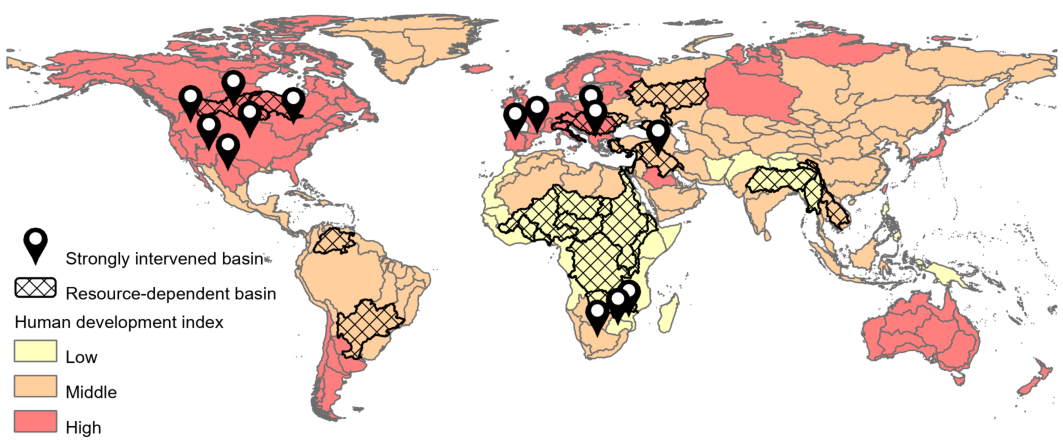
\includegraphics[width=\linewidth]{../../figures/main/map.pdf}
	\caption{
		\textbf{The Human Development Index of the world's great river basins, and the major problems facing some basins.}
		Overdependence on water resources for economic development in some basins, and high levels of human modification in others that have disrupted ecosystem structure. Data resources: Human Development Index in each basin refers from \cite{linkeGlobalHydroenvironmentalSubbasin2019}, strongly intervened basins and resource-dependent basins are come from Transboundary River Basins report by United Nations Environment Programme \url{http://geftwap.org/publications/river-basins-technical-report} \cite{unep-dhiTransboundaryRiverBasins2016}.
	}
	\label{fig:traps}
\end{figure}

% 世界各大流域面临的问题。资源开发早期容易陷入资源陷阱;流域发展后期容易陷入结构陷阱。
According to cases all around the world, big river basins often face resource dilemmas after resources-dependent developments, while highly developed ones need to resolve structural problems more often (Figure~\ref{fig:traps}).
% 黄河流域的发展过程,资源开发P2阶段陷入了资源陷阱(表现形式 xxx)。
In the YRB as an example, after the successive exploitation of agriculture (from P1 to P2, refers from natural cycle to a local cycle), industry and services, the water resource extraction rate has reached $79\%$, far exceeding the internationally recognized warning threshold of $40\%$. The resource dilemma revealed after the regime shift, with severe runoff outages and groundwater depletion of the Yellow River (\textit{SI Appendix} Fig. S8).
% 后来摆脱了资源陷阱(表现形式 xxx)。
To get rid of the resource dilemma, a clear transformation towards integrated basin management proposed, with several management practices. 
% 一段有关87分水方案的介绍
The most important of these is the “87 Water Allocation Scheme”, which adopts a top-down approach in allocating water resources to all regions and sectors \cite{wangThirtyYearsYellow2018}. Since then, the scheme has been revised and refined, and a comprehensive water resources utilization system has gradually been formed that takes the basin scale into account \cite{wangThirtyYearsYellow2018}. 
These integrated management practices made the utilization of water resources into a regime of unified scheduling since the P3 in the Yellow River Basin, to escape from the resource dilemma. 
% 资源困局可能普遍存在
Since similar phenomena occurred in Mississippi and Indus River Basins, the fact that the accelerated development has been followed by water scarcity and a series of ecological problems shows that the resource dilemmas is pervasive in the transition trajectory, especially from natural cycle to regional cycle 
\cite{bestAnthropogenicStressesWorld2019,cummingResilienceBigRiver2011}.
% 通过协同治理来摆脱困局也普遍存在
Similarly, many of the world's major river basins have eventually moved towards a system of integrated governance, especially for trans-boundary rivers (e.g. Danube and Mekong River), where water resources are in need of collaborative governance \cite{bodinCollaborativeEnvironmentalGovernance2017,unep-dhiTransboundaryRiverBasins2016}.

% 此外,即使发展极大提升了用水效率,黄河流域的困境也并没能完全解决。
In addition, further dilemmas of the YRB has not been completely solved though water use efficiency greatly improved by development.
% 展望:未来还可能陷入结构陷阱,(表现形式:用水效率悖论的同时,倾向性停滞,灵活性进一步降低,)
% Therefore, basins still in need of further transformations according to changes within the transition cycle of water utilization. 
Firstly, in line with paradox of irrigation efficiency, significant improvement in agricultural irrigation efficiency has been accompanied by re-growths in irrigated area, still resulting in an unabated and weak upward trend in water resources stress \cite{graftonParadoxIrrigationEfficiency2018}.
% 水资源压力仍在增大,而节水能力已经进入瓶颈,倾向性贡献减少)
Secondly, the changing priority between non-provisioning (i.e. industry or services) and provisioning (i.e. domestic and irrigation water use) may rigidify the flexibility of water use, since domestic water use and thermal water use growth rapidly (supplementary Fig. S4). 
% 下一步:可以通过统一调控,调整格局来调整结构,突破结构陷阱。
% 总结:整个流域需进一步转型与适应,以实现高质量发展。
Typically, these may lead to a reduction in resilience of basins and leave highly coupled human-water systems facing greater vulnerability to collapse --as a structural dilemma \cite{cummingResilienceBigRiver2011}. Therefore, based on the identification of current phases and development dilemmas by the transition framework, further transformative governance is still needed to achieve a high-quality sustainable development of the basin, because development is not a panacea for the dilemmas \cite{scoonesTransformationsSustainabilityCombining2020a}.




%tag 研究方法
\matmethods{
Here, we constructed the Integrated Water Resources Utilization (IWRU) Index which consists of three dimensions and identified the regime in the changes of the index over time by change points detection. Finally, the contribution to changes of IWRU index along with each main indicators were calculated separately for each regime (i.e. period). 
	
	\subsection*{Integrated Water Resources Utilization (IWRU) Index}
	The Integrated Water Resources Utilization (IWRU) Index consists of three dimensions (stresses, priority and configurations, denoted by sub-indicators correspondingly). Assuming they have equal weights, we log-transformed and standardized the three sub-indicators for elimination of differences between indicators. It means for each indicator $I_{sub}$, we performed:
	$$ I' = log(I_{sub}) $$
	$$ I = (I' - I'_{min}) / (I'_{max}-I'_{min})$$
	where $I$ is standardized series for $I_{sub}$.
	Then, since we assumed different relationships between development and sub-indicators, we added them together in equal weights:
	$$ IWRU = \sum_{i}^3 I'_i $$
	where $i$ is stress, priority or configuration, and $I'_i$ is standardized sub-indicator of them. A brief description of the sub-indicators used to measure each dimension follows (see SI Methods. S3 for more details).

	\subsubsection*{Sub-indicator of Stresses}
	Humans use technology to continuously manage water resources, so a simple physical water scarcity index cannot reasonably assess water scarcity in the evolution and transition of socio-water systems. Therefore, we refer to the scarcity-flexibility-variability (SFV) water stress index proposed in Qin et al., 2019 to evaluate water scarcity in the basin. The index takes into account management measures (such as the construction of reservoirs) and the impact of changes in the industrial structure of water use on the evaluation of water scarcity \cite{qinFlexibilityIntensityGlobal2019}.

	To apply this method, we need to combine three metrics following: 
	
	First for scarcity, $A_{i, j}$ is the total water consumption as a proportion of regional multi-year average runoff volume, in year $j$ and region $i$:
	$$ A_{i, j} = \frac{WU_{i,j}}{R_{i, avg}} $$
	Second for flexibility, $B_{i, j}$ is the inflexible water use $WU_{inflexible}$ (i.e. for thermal power plants or humans and livestock) as a proportion of average multi-year runoff, in year $i$ and region $j$:
	$$ B_{i, j} = \frac{WU_{inflexible}}{R_{i, avg}} $$
	Finally for variability, the capacity of the reservoir and the positive effects of storage on natural runoff fluctuations are also considered.
	$$ C_i = C1_i * (1 - C2_i) $$
	$$ C1_{i, j} = \frac{R_{i, std}}{R_{i, avg}} $$
	$$ C2_{i} = \frac{RC_{i}}{R_{i, avg}}, \ if RC < R_{i, avg} $$
	$$ C2_{i} = 1, \ if RC >= R_{i, avg} $$
	In all the equations above, $R_{i, avg}$ is the average runoff in region $i$, $RC_i$ is the total storage capacities of reservoirs in the region $i$, $R_{i, std}$ is the standard deviation of runoff in the region $i$.

	Finally, assuming three metrics (scarcity, flexibility and variability) have the same weights, we can calculate $SFV$ index after normalizing them:
	$$ V = \frac{A_{normalize} + B_{normalize} + C_{normalize}}{3} $$
	$$ a = \frac{1}{V_{max} - V_{min}}; $$
	$$ b = \frac{1}{V_{min} - V_{max}} * V_{min} $$
	$$ SFV = a * V + b $$

	\subsubsection*{Sub-indicator of priority}
	To priority, we use non-provisioning shares of water use as an indicator. While provisional water use ($WU_{pro}$) includes domestic, irrigated and livestock water uses, the non-provisioning water use ($WU_{non-pro}$) includes industrial and urban services water uses. Then, we can calculate the non-provisioning shares by:
	$$ NPS_{ij} = \frac{WU_{indirect, i, j}}{WU_{direct, i, j} + WU_{undirect, i, j}} $$

	\subsubsection*{Sub-indicator of configurations}
	To description of configurations between regions or sections, we designed an indicator by imitation of information entropy (Allocational Entropy Metric, see supplementary document: Methods S4). Assuming the most egalitarian water allocation is assumed to be that each region or sectoral development utilizes the same proportion of water resources (the case of maximum entropy). The ratio between the actual water allocation entropy and this maximum entropy is the allocation entropy index.
	$$ ratio = \frac{Entropy}{Entropy_{max}} $$
	where $Entropy$ and $Entropy_{max}$ are entropy and maximum entropy of water distributions, respectively. They can be calculated by:
	$$ Entropy = \sum_{i=1}^n \sum_{j=1}^m -log(p_{ij}) * p_{ij} $$
	$$ Entropy_{max} = n * \sum_{j=1}^m -\frac{p_j}{n} * log(\frac{p_j}{n}) $$ 
	where $p_j$ and $p_ij$ are proportions of water use in sector $j$ and region $i$:
	$$ p_j = \frac{\sum_{i=1}^n WU_j}{\sum_{i=1}^n WU} $$
	$$ p_{ij} = \frac{WU_{ij}} {\sum_{i=1}^n \sum_{j=1}^m WU_{ij}} $$
	where $n$ is the total number of regions ($n=4$ here, see supplementary Methods. S1) and $m$ is the total number of sectors ($m=4$ here, see supplementary Methods. S2).

	\subsection*{Change points detection}
		The method makes no assumptions about the distribution of the data and detects breakpoints based solely on the probability of the data coming from different distributions before and after the breakpoint.
		The approach after Pettitt (1979) is commonly applied to detect a single change-point in hydrological series or climate series with continuous data \cite{pettittNonParametricApproachChangePoint1979}. It tests the $H0$: The variables follow one or more distributions that have the same location parameter (no change), against the alternative: a change point exists. The non-parametric statistic is defined as:
	
		$$ K_t = max|U_{t, T}|$$
		where:
		$$ U_{t, T} = \sum_{i=1}^t\sum_{j=t+1}^T sgn(X_i - X_j) $$
	
		The change-point of the series is located at $K_T$, provided that the statistic is significant. We use 0.001 as the threshold of p-value, which means the probability of a statistically significant change-point judgment being valid is more than $99.9\%$. Since this method only can return one significant change point, we repeat it Until all significant change points were detected.
	
	% 计算贡献度
	\subsection*{Contribution decomposition}
	\subsubsection*{Change contributions}
		We have decomposed the amount of variation in each index at different stages in order to observe the contribution of each influencing factor to them. Use Integrated Water Resources Utilization (IWRU) Index as an example, which influenced by three dimensions: stress ($S$), priority ($T$) and configuration ($P$) (indicated by their own index respectively, see Water utilization regime index and supplementary Methods. S3):
		$$ IWRU = T * P * S ^ {-1} $$
		Take the logarithm of both sides then, we get:
		$$ ln(IWRU) = ln(S) + ln(T) - ln(P) $$
		Since the changes of IWRU $\Delta IWRU$ can be expressed as $\Delta IWRU = ln(IWRU_2) - ln(IWRU_1)$, where $IWRU_2$ and $IWRU_1$ are ending and beginning values of IWRU in a certain time period, combining the above equations we can get:
		$$ \Delta IWRU = ln(\frac{S_1}{S_2}) + ln(\frac{T_2}{T_1}) + ln(\frac{P_2}{P_1}) = -\Delta S + \Delta T + \Delta P $$
		Then, we can calculate contributions $C_F$ of a certain factor $F$ in a certain period by:
		$$ C_{F} = \frac{|\Delta C_{F}|}{\Delta IWRU}$$
		
	\subsubsection*{Net contributions}
		% TODO 这里补充 ”net contribution“ 的方法介绍
		}

\showmatmethods{} % Display the Materials and Methods section

\acknow{Please include your acknowledgments here, set in a single paragraph. Please do not include any acknowledgments in the Supporting Information, or anywhere else in the manuscript.}

\showacknow{} % Display the acknowledgments section

% Bibliography
\bibliography{my-papers}
	
\end{document}